The following section deals with the training process of YOLO and MobileNetV2-UNet.
For both networks similar experiments were performed each sub-experiment was repeated three times each with a different seed.
The used seeds were: $\{42, 1337, 0xDEADBEEF\}$

First an initial learning rate search was performed, here six to seven learning rates were tested on the basic dataset.
The basic dataset is the default train/valid/test split (table \ref{tab:data_distribution} and \ref{tab:yolo_classes}) without any pre-augmentations of the training set.
The best performing learning rate is then taken as the baseline for the following experiments.

The second conducted experiment is a search for the perfect configuration of so called offline augmentations.
Offline augmentations are a 90\textdegree, 180\textdegree and a 270\textdegree  rotation of the original image, as well as a horizontal flip and again three rotations of the flipped image.
Furthermore, as has been described in section \ref{sec:data}, for some images a mask has been created, which is projected on different checkered background images to increase the amount of those.
This offline augmentation is referred to as projection.
The search for the best configuration is performed by taking all possible configuration of those three offline augmentations.

Afterwards, an ablation study is performed for various augmentations, with different parameters.
The augmentations in that study are also referred to as online augmentations, since they are performed at training time.
The occurrence probability of those augmentations is set to 50\%.
Since, the augmentations slightly differ for each network they are explained in the respective subsection.

The last experiment step is formed by a fine tuning step, where a grid search was performed.
The grid search always utilizes the best performing offline and online augmentations and consists of various learning rates, batch sizes and other network specific parameters.

The evaluation of each experiment is done by comparing the mean and standard deviation of each experiment, if the mean is higher, in almost all cases this configuration is considered to be superior to another one, the standard deviation should still remain in a reasonable area.

\subsection{YOLOv4-Tiny}

To perform any experiments with \ac{YOLO} first an initial configuration was defined.
This configuration is given in \ref{tab:initial_yolo_config}, it consist of a fixed batch size of $64$, the \ac{CIoU} loss as described in section \ref{sec:yolo}. \ac{SGD} with momentum was used as the optimizer with a momentum rate of $0.9$.

\begin{table}[H]
\footnotesize
\begin{center}
\begin{tabular}{|l|l|}

\hline
\textbf{Batch Size} & $64$\\
\hline
\textbf{Loss} & CIoU \\
\hline
\textbf{Optimizer} & SGD with Momentum \\
\hline
\textbf{Momentum} & $0.9$ \\
\hline
\textbf{Burn in} & 1000 steps \\
\hline
\textbf{Dataset} & Base Dataset \\
\hline

\end{tabular}
\caption{The initial training configuration for the experiments performed with the YOLO network.}
\label{tab:initial_yolo_config}
\end{center}
\end{table}

Redmon et al. have pointed out that training \ac{YOLO} is unstable, when the full learning rate is applied without proper scheduling \cite{yolov2}.
This was also tested in this thesis and can be confirmed, all learning rates which were tested in the initial learning rate search diverged when used without a scheduling mechanism.
The proposed scheduling function by Redmon et al., which is still used in the current \ac{YOLOv4} \cite{yolov4}, is given by the following formula:

\begin{equation}
    lr(step) =
    \begin{cases}
        lr_{base} * (\frac{step}{burn\_in})^4 & \textbf{if } step < burn\_in\\
        lr_{base}                             & \textbf{else}
    \end{cases}
\end{equation}

Where a step is defined as one whole batch and the $burn\_in$ is set to $1000$ steps.

All trained experiments were optimized for a slightly changed COCO mAP metric.
COCO uses a $mAP0.5:0.95:0.05$, while in this thesis $mAP0.5:0.75:0.05$ is used, since an \ac{IoU} of $0.75$ is considered to be enough for the whole system to work properly in most circumstances.
All experiments are optimized for this metric, which means that at every step the mAP is calculated for the whole validation set and if the mAP is better than the previously calculated mAP, the weights of the network are stored and used for further evaluation.

\subsubsection{Experiment: Initial Learning Rate Search}

The first experiment was executed to find an initial learning rate for further experiments.
The parameters for the network were set to the ones in table \ref{tab:initial_yolo_config} and kept for all training runs.
The results of the training runs can be found in figure \ref{fig:yolo_lr_experiment_results}, where the mean of mAP for the three performed runs is shown for each learning rate.
The full results of the learning rate search with classwise performance can be found in table \ref{tab:yolo_init_lr_results} in the appendix.
It can be observed that the learning rate $0.001$ has the highest \ac{mAP}, therefore it is selected as the default learning rate for further experiments.
This experiment has shown that the text class and especially the arrow classes showed consistently bad performance over all learning rates.

\begin{figure}
\begin{center}
    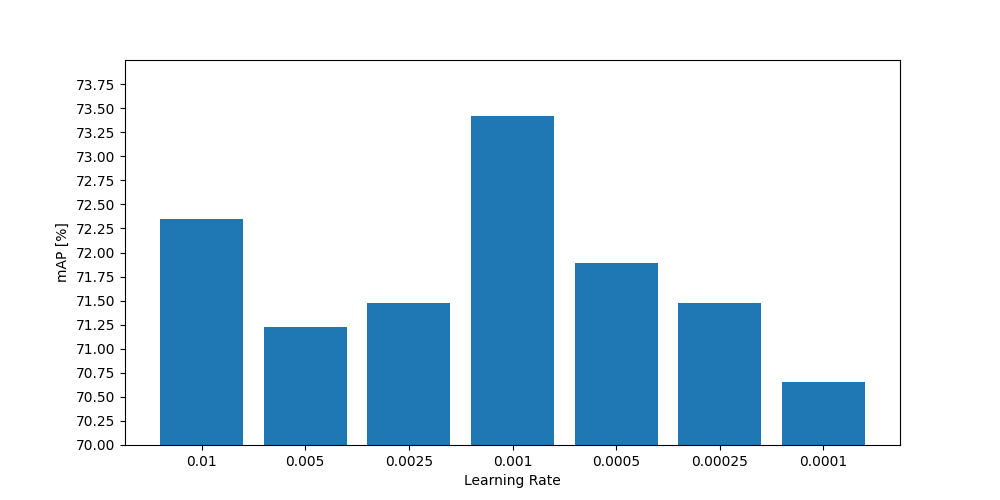
\includegraphics[width=16cm]{imgs/yolo_lr_experiment.png}
    \caption{The results of the initial learning rate search shown on the validation set, as the mean of the mAPs of three separate training runs.}
    \label{fig:yolo_lr_experiment_results}
\end{center}
\end{figure}


\subsubsection{Experiment: Offline Augmentations}

This experiment was conducted to find the optimal configuration of offline augmentations, where the offline augmentations are projection (copy-paste augmentation \cite{copypaste_aug}), three 90\textdegree\ rotations and a horizontal flip.
If both the rotation and the flip augmentation are selected at the same time, then additionally the flipped image is rotated three times.
Again for all runs the YOLO configuration from the previous experiment was used, but additionally now the learning rate is set to the best performing one from the learning rate search experiment.
The new configuration can be found in table \ref{tab:yolo_offline_aug_config}.

\begin{table}[H]
\footnotesize
\begin{center}
\begin{tabular}{|l|l|}

\hline
\textbf{Learning Rate} & $0.001$ \\
\hline
\textbf{Batch Size} & $64$\\
\hline
\textbf{Loss} & CIoU \\
\hline
\textbf{Optimizer} & SGD with Momentum \\
\hline
\textbf{Momentum} & $0.9$ \\
\hline
\textbf{Burn in} & 1000 steps \\
\hline
\textbf{Dataset} & Depending on experiment configuration \\
\hline

\end{tabular}
\caption{The training configuration for the offline augmentation experiment, where the learning rate is set to the best performing learning rate from the learning rate search and the data is pre-augmented with the respective experiment configuration.}
\label{tab:yolo_offline_aug_config}
\end{center}
\end{table}

The full results with classwise \ac{AP} can be found in the appendix in table \ref{tab:yolo_offline_aug_results}.
\begin{figure}
\begin{center}
    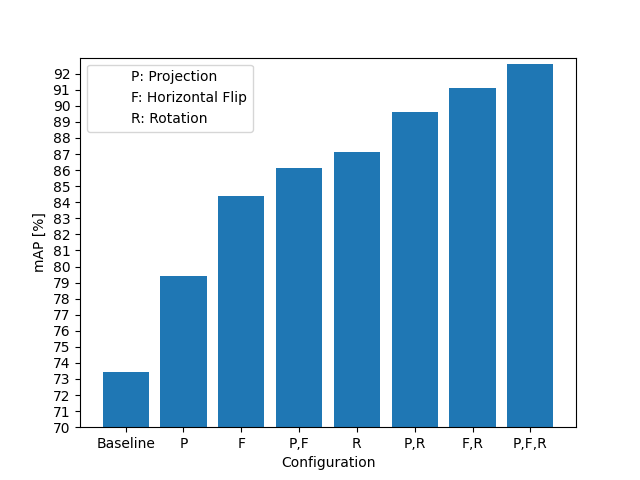
\includegraphics[width=14cm]{imgs/yolo_offline_aug_experiment.png}
    \caption{The results of the offline augmentation with the different offline augmentation configurations compared with the results of the best performing learning rate (baseline). When rotation and flip are enabled simultaneously the flipped image also gets rotated three times by 90\textdegree. Results are given as the mean of the mAP of three separate training runs.}
    \label{fig:yolo_offline_aug_results}
\end{center}
\end{figure}

The results for this experiment are also shown in figure \ref{fig:yolo_offline_aug_results}, where a clear trend emerges.
When looking at the results as an ablation it can be seen that each offline augmentation brought an increase in \ac{mAP} and the combination of those too.
Rotation has an absolute increase in mAP, when compared to the baseline (the best performing learning rate), of $13.725\%$, flip shows an increase of $11.000\%$ and the copy-paste augmentation shows an increase of $5.988\%$.
The best configuration is, as expected, the one where all three augmentations are used simultaneously and it has an increase in \ac{mAP} of $19.163\%$.
When specifically comparing the results of the best performing configuration with the baseline, it can be observed that all \ac{ECC} classes have reached a \ac{mAP} greater than $90\%$.
The text and arrow classes have also greatly increased.
Text shows an increase of $24.485\%$ and the mean over the arrow classes shows an increase of $47.988\%$, however those two classes are still not near the desired performance observed at the \acp{ECC}.
It should be pointed out that especially the increase in the text class is very interesting, because this is the only class which is not rotation and flip invariant, i.e. flipping a diode produces again a diode (also for the human perception), but with a different orientation, however flipping a text will produce something no more really interpretable (at least for the human perception).
An explanation why there is still an increase in recognition performance could be that the network starts learning blob like regions, which are located near \acp{ECC}, instead of specific features of the different texts.


\subsubsection{Experiment: Online Augmentations}

The next presented experiment is an ablation study performed on various augmentations and parameters for those augmentations.
Since these augmentations are performed at runtime, they are also called online augmentations.
As mentioned, the images were augmented utilizing the open-source library albumentations \cite{albumentation}.


\subsubsection{Experiment: Grid Search}

\subsection{MobileNetV2-UNet}

\subsubsection{Experiment: Initial Learning Rate Search}

\subsubsection{Experiment: Offline Augmentations}

\subsubsection{Experiment: Online Augmentations}

\subsubsection{Experiment: Grid Search}

\subsection{MobileNetV2-UNet}
